En esta práctica se calcula la cinemática inversa para manipuladores bidimensionales. Es decir, se obtienen las variables articulares necesarias para alcanzar un punto objetivo en el plano. Para ello, se emplea el algoritmo iterativo \textit{Cyclic Coordinate Descent} (CCD).

\bigskip Se caracteriza el robot mediante sus articulaciones, prismáticas o de revolución, y sus parámetros de Denavit-Hartenberg theta y a (al encontrarnos en 2D solo hay 2 parámetros).
Al ejecutar el script se indica las coordenadas del punto objetivo para el extremo del robot, y se obtienen las variables articulares necesarias para alcanzar dicho punto.

\section{Código Implementado}

\subsection{Análisis}
El script proporcionado contiene muchas de las funciones necesarias, sin embargo, se deben implementar varias funciones para poder calcular la cinemática inversa. Principalmente, se debe implementar la lógica del CCD. Se realiza un cálculo para cada articulación desde el extremo final (EF) hasta el origen del robot, actualizando su valor y recalculando la cinemática directa. Al finalizar, se comprueba la distancia al punto objetivo, si es menor a la tolerancia indicada (umbral de convergencia epsilon), se finaliza. En caso contrario, se itera hasta conseguir una aproximación tolerable, o que se detecte la imposibilidad de convergencia.
\begin{itemize}
   \item \texttt{Detección del tipo de articulación} se distingue entre articulaciones prismáticas y de revolución.
   \item \texttt{Cálculo de las articulaciones prismáticas} Para calcular la distancia que se incrementa o decrementa la articulación, se calcula la distancia entre el extremo del robot y el punto objetivo, proyectada sobre la recta de movimiento de la articulación prismática. Esto se consigue realizando el producto del vector unitario $\vec{u}$, que representa la dirección de la variable prismática, y el vector $\vec{v}$, que une el extremo del robot y el punto objetivo. El vector $\vec{u}$ se obtiene sumando los ángulos de todas las articulaciones previas a la actual, y calculando el seno y coseno del resultado. 
   \item \texttt{Cálculo de las articulaciones de revolución} se calcula el ángulo en el que se debe modificar la articulación calculando la diferencia entre el vector $\vec{v}$, que une la articulación de rotación y el punto extremo EF, y el vector $\vec{w}$, que une la articulación de rotación y el punto objetivo. Para ello, se normalizan ambos vectores y se calcula la diferencia entre sus arcotargentes. En la práctica, se emplea la función \textit{math.atan2} ya que se encarga de realizar las comprobaciones necesarias de cuadrantes.
   \item \texttt{Corrección de ángulo de rotación} se corrige el ángulo calculado para que se encuentre en el rango $[-\pi, \pi]$.
   \item \texttt{Límites} se implementan límites inferiores y superiores para cada articulación. En caso de que el nuevo valor de las variables articulares este por debajo, se emplea el límite inferior, y si está por encima, el superior.
\end {itemize}

En las figuras~\ref{chapter:code_ccd1} y ~\ref{chapter:code_ccd2} se muestra el código implementado para el CCD.
\begin{figure}[htb]
   \centering
   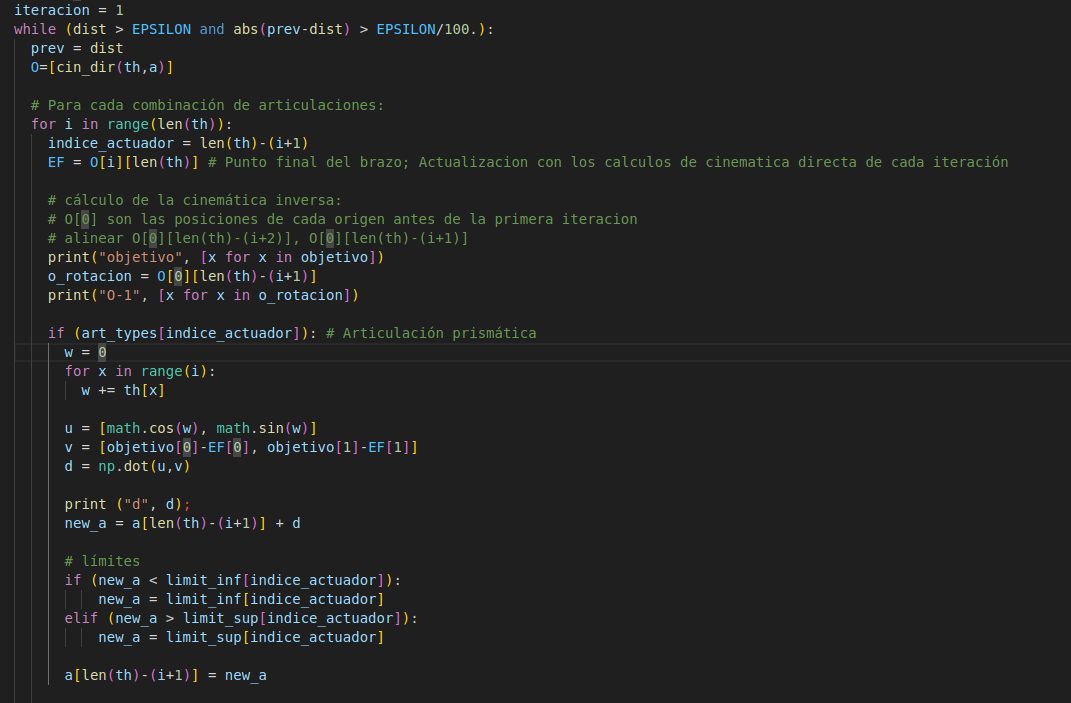
\includegraphics[width=1\linewidth]{images/ccd_1.png}
   \caption{Código del CCD para articulaciones prismáticas}
   \label{chapter:code_ccd1}
\end{figure}
\begin{figure}[htb]
   \centering
   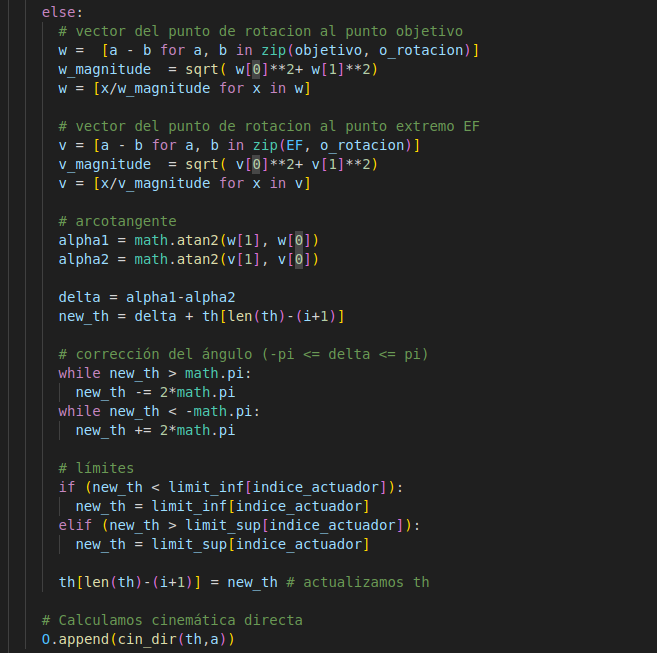
\includegraphics[width=1\linewidth]{images/ccd_2.png}
   \caption{Código del CCD para articulaciones de revolución}
   \label{chapter:code_ccd2}
\end{figure}

\subsection{Complejidad}
Para la cinemática inversa, se realiza una aproximación iterativa, en la que en cada iteración se debe calcular cada articulación.
Tras actualizar cada articulación, se debe recalcular la cinemática directa.
Es decir, para N articulaciones en una iteración se debe calcular N veces la cinemática directa. Como se dijo en el anterior capítulo, la cinemática directa es lineal respecto al número de articulaciones, por lo que la complejidad de la cinemática inversa es cuadrática $\sim O(N^2) $.

\subsection{Fé de erratas}
El código entregado en prácticas contenía un pequeño pero importante error. En la detección del tipo de articulación, se estaba empleando un índice incorrecto: se recorría en el orden inverso, de origen a extremo. Esto provocaba que se detectaran las articulaciones de forma incorrecta. No se había detectado en la entrega ya que los ejemplos provados eran simétricos en ese sentido. Se ha corregido este problema, y como se puede observar más adelante, el programa funciona correctamente en todos los casos.

%%%%%%%%%%%%%%%%%%%%%%%%%%%%%%%%%%%%%%%%%%%%%%%%%%%%%%%%%%%%%


\section{Mejoras}
Se ha implementado una sola mejora, la lectura de JSON.

\subsection{Lectura de JSON}
Se leen las características de cada articulación desde un fichero JSON. Cada articulación se caracteriza por su tipo (rotacion o primastica), sus parámetros de Denavit-Hartenberg (th y a),
y sus límites inferiores y superiores, expresados en unidades de longitud o radianes.

En el fichero, las articulaciones se indican en orden desde el origen hasta el extremo, siendo la primera la más cercana al origen.

En la figura \ref{chapter:code_ccd3} se muestra el código implementado para la lectura de JSON. En la figura \ref{chapter:ccd_json1} se observa un ejemplo de fichero JSON para un robot con una articulación de rotación, otra prismática, y otra de revolución.
\begin{figure}[htb]
   \centering
   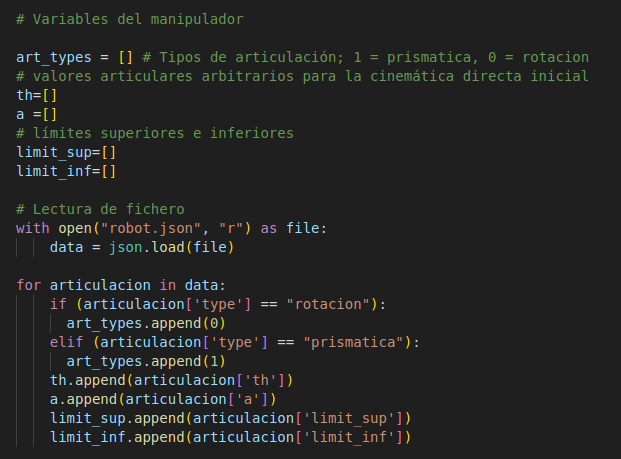
\includegraphics[width=.8\linewidth]{images/ccd_3.png}
   \caption{Código para la lectura de JSON}
   \label{chapter:code_ccd3}
\end{figure}
\begin{figure}[htb]
   \centering
   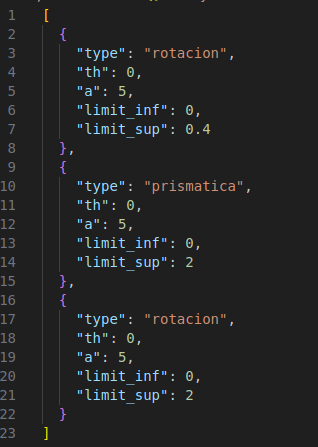
\includegraphics[width=.4\linewidth]{images/ccd_json1.png}
   \caption{Ejemplo de fichero JSON para un robot de 3 articulaciones}
   \label{chapter:ccd_json1}
\end{figure}


\subsection{Propuestas}
Actualmente solo se consideran las dimensiones iniciales del robot para la visualización. Sería interesante considerar también las coordenadas del punto objetivo para garantizar que se visualiza correctamente.
%%%%%%%%%%%%%%%%%%%%%%%%%%%%%%%%%%%%%%%%%%%%%%%%%%%%%%%%%

\section{Ejemplo}
En la figura \ref{chapter:ccd_json2} se muestra un ejemplo de fichero JSON con las características de un robot de 5 articulaciones.
\begin{figure}[htb]
   \centering
   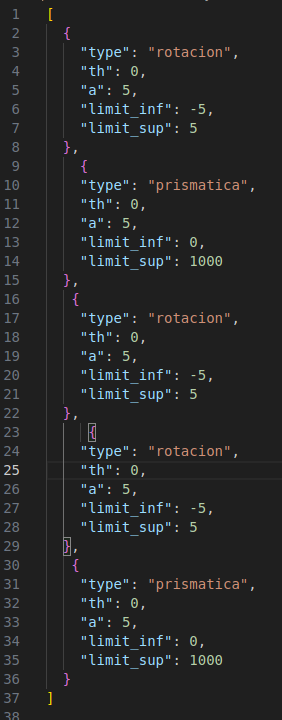
\includegraphics[width=.4\linewidth]{images/ccd_json2.png}
   \caption{Ejemplo de fichero JSON para un robot de 5 articulaciones}
   \label{chapter:ccd_json2}
\end{figure}

\subsection{Ejecución 1}
En la figura \ref{chapter:ccd_ejemplo1} se muestra la primera iteración del algoritmo sobre el robot descrito considerando como objetivo el punto 10,10.
En la figura \ref{chapter:ccd_ejemplo2} se muestra la última iteración del algoritmo, en la que se ha alcanzado el umbral de convergencia. En este caso, se consigue converger en solo 2 iteraciones.

\begin{figure}[htb]
   \centering
   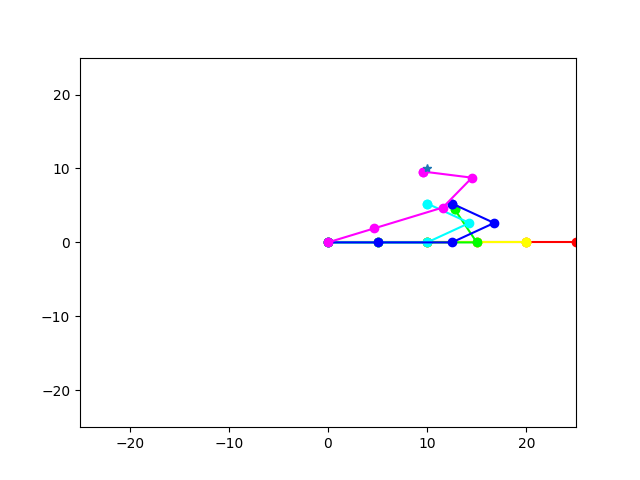
\includegraphics[width=.8\linewidth]{images/ccd_5.png}
   \caption{Primera iteración para objetivo 10,10}
   \label{chapter:ccd_ejemplo1}
\end{figure}
\begin{figure}[htb]
   \centering
   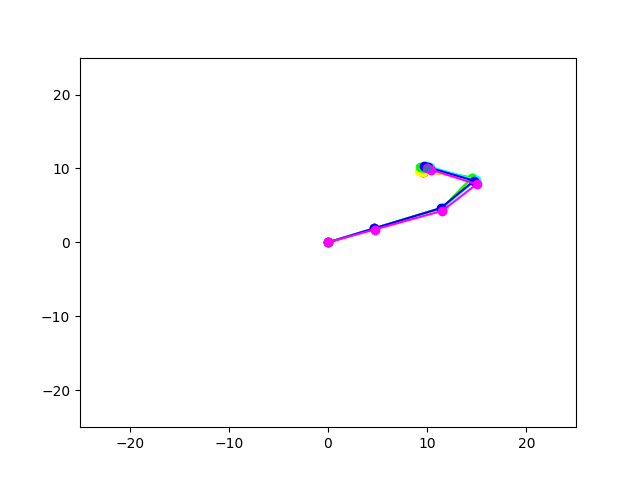
\includegraphics[width=.8\linewidth]{images/ccd_6.png}
   \caption{Última iteración para objetivo 10,10}
   \label{chapter:ccd_ejemplo2}
\end{figure}

\subsection{Ejecución 2}
En la figura \ref{chapter:ccd_ejemplo3} se muestra la primera iteración del algoritmo sobre el robot descrito considerando como objetivo el punto -20,-20.
En la figura \ref{chapter:ccd_ejemplo4} se muestra la última iteración del algoritmo, en la que se ha alcanzado el umbral de convergencia. En este caso, se consigue converger en 5 iteraciones.
Se aprovecha este ejemplo para estudiar la influencia del valor del umbral de convergencia en el número de iteraciones necesarias. El epsilon empleado por defecto es de 0.01, cambiándolo a 0.1, se converge en menos iteraciones, 4 en este caso. 
Se comprueba por tanto empíricamente que un umbral mayor implica menos iteraciones, pero también una menor precisión en el resultado obtenido.
\begin{figure}[htb]
   \centering
   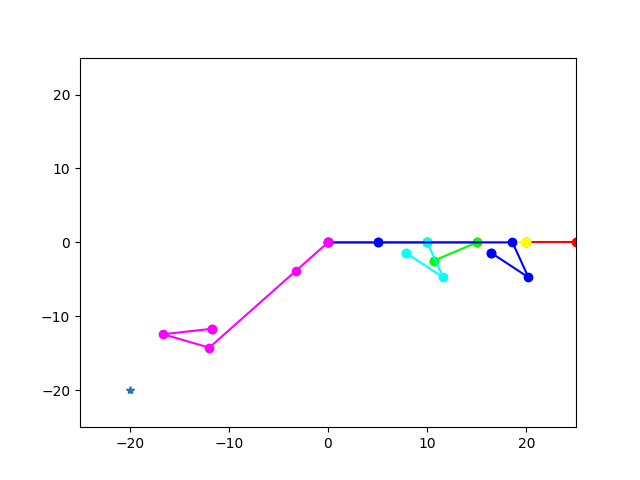
\includegraphics[width=.8\linewidth]{images/ccd_7.png}
   \caption{Primera iteración para objetivo -20,-20}
   \label{chapter:ccd_ejemplo3}
\end{figure}
\begin{figure}[htb]
   \centering
   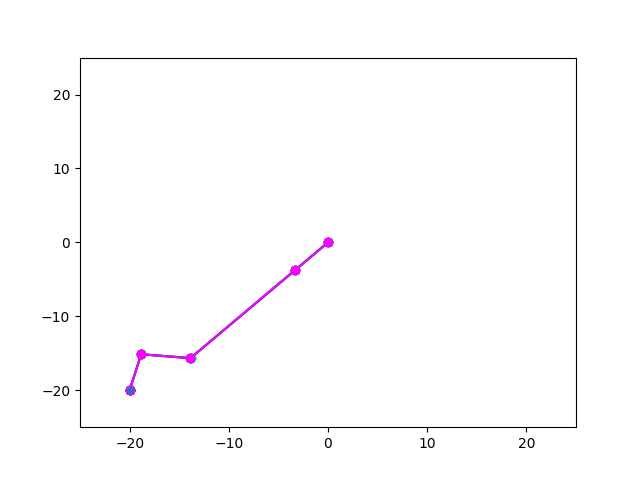
\includegraphics[width=.8\linewidth]{images/ccd_9.png}
   \caption{Última iteración para objetivo -20,-20}
   \label{chapter:ccd_ejemplo4}
\end{figure}


\subsection{Ejecución 3}
Empleando el robot de la figura \ref{chapter:ccd_json1} se comprueba que se detectan los casos en los que no se converge, esto es, no existe solución para alcanzar el punto objetivo con el robot dado.

La figura \ref{chapter:ccd_ejemplo5} muestra la última iteración para el punto objetivo 10,10. Por los límites establecidos, el robot solo puede alcanzar puntos a un radio de 12 unidades, por lo que no puede llegar al punto 10,10.
En la figura \ref{chapter:ccd_ejemplo6} se muestra la salida por consola indicando que no se ha podido converger, ya que se detecta que la distancia al objetivo ha disminuido menos de epsilon/100.
\begin{figure}[htb]
   \centering
   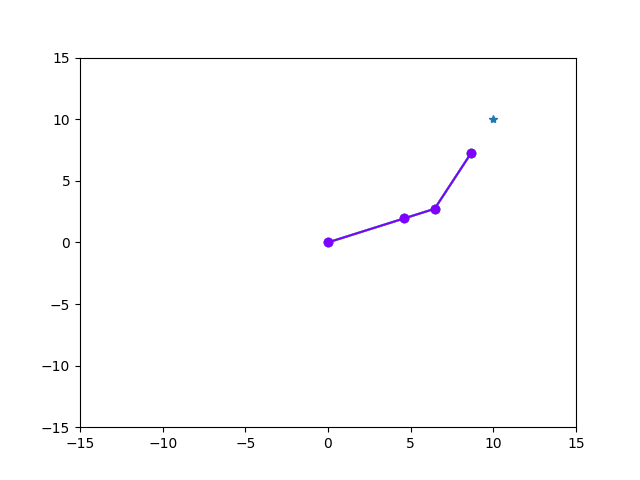
\includegraphics[width=.8\linewidth]{images/ccd_10.png}
   \caption{Última iteración para objetivo 10,10}
   \label{chapter:ccd_ejemplo5}
\end{figure}
\begin{figure}[htb]
   \centering
   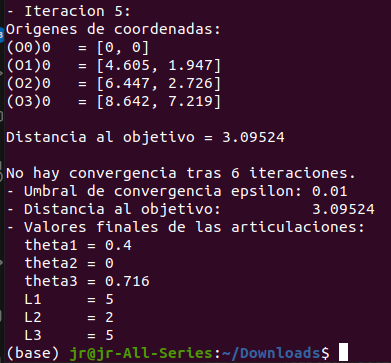
\includegraphics[width=.6\linewidth]{images/ccd_11.png}
   \caption{Salida por consola cuando no converge}
   \label{chapter:ccd_ejemplo6}
\end{figure}


\section{Conclusions}
We have implemented the inverse kinematics for a 2D manipulator, using the CCD algorithm. The immplementation considers both prismatic and revolute joints, for wich we admit lower and upper limits.
We have studied the effects of different convergence thresholds, seen that a higher threshold implies less iterations but also less precision.
Also, we have studied the complexity of the inverse kinematics with the CCD algorithm. We have seen that it is quadratic, as it is a iterative process in which we must calculate the direct kinematics for each articulation in each iteration.

\bigskip We can conclude that the inverse kinematics are generally more complex and expensive than the direct kinematics, as an exact approach is not always valid because for some configurations there may exist multiple or none solutions. 

